\chapter{Cơ sở lý thuyết và nghiên cứu liên quan}
\label{chap:co-so}

\section{Định vị lỗi dựa trên phổ độ phủ và lỗi ngữ nghĩa}
\label{sec:sbfl}

SBFL gán cho mỗi dòng $s$ một điểm nghi ngờ tính từ ma trận độ phủ (kiểm thử $\times$ dòng). Với $e_f(s)$, $e_p(s)$
là số kiểm thử thất bại, thành công chạy qua $s$ và $n_f(s)$ là số kiểm thử thất bại không chạy qua $s$, công thức
Ochiai~\cite{abreu2009} dùng trong tiểu luận là
\begin{equation} \mathrm{Ochiai}(s) = \frac{e_f}{\sqrt{(e_f+n_f)\,(e_f+e_p)}}. \label{eq:ochiai} \end{equation}
Các dòng được xếp giảm dần theo điểm; dòng không kiểm thử thất bại nào chạy qua ($e_f = 0$) không được xếp hạng.

\textbf{Chỉ số đánh giá.} Hạng của lỗi là hạng tốt nhất của một dòng lỗi chuẩn, và
\begin{equation} \mathrm{Acc@}k = \frac{1}{|\mathcal{P}|} \sum_{p \in \mathcal{P}} \mathbb{1}\!\left[\,\mathrm{rank}_p \le k\,\right], \label{eq:acck} \end{equation}
trong đó $\mathcal{P}$ là tập chương trình \emph{cố định}: chương trình mà công cụ không chạy được vẫn nằm trong mẫu số
và tính là trượt. Khi nhiều dòng cùng điểm, tiểu luận dùng \emph{hạng trung bình} của nhóm hòa theo khuyến
nghị~\cite{pearson2017,desouza2016}; cách chấm của tác giả SemLoc lấy vị trí đầu. Chỉ số chính chấm khớp đúng dòng;
\emph{Acc@1 nới lỏng} chấp nhận thêm dòng kề khi hai dòng là đầu một câu lệnh ghép và câu lệnh nó bảo vệ
(Chương~\ref{chap:ket-qua}).

\label{sec:loi-ngu-nghia}%
Lỗi ngữ nghĩa làm chương trình tính sai giá trị trong khi vẫn chạy qua cùng các câu lệnh như khi đúng. Khi cả
kiểm thử thành công và thất bại đều chạy qua dòng lỗi, $e_p(s) > 0$ kéo điểm Ochiai của dòng lỗi xuống ngang các dòng
xung quanh và SBFL gần như đoán mò trong phạm vi hàm (Hình~\ref{fig:sbfl-mu}). Để phân tích theo loại lỗi, tiểu luận gán nhãn tự động theo độ phủ của dòng lỗi chuẩn:
\emph{lỗi ngữ nghĩa} khi dòng lỗi được ít nhất một kiểm thử thất bại và một kiểm thử thành công chạy qua;
\emph{lộ qua độ phủ} khi chỉ kiểm thử thất bại chạy tới; \emph{không thực thi} khi không kiểm thử thất bại nào chạy tới
(thường do nhãn đặt sai hoặc ở dòng trống). Nhãn được tính lại theo bộ dòng lỗi chuẩn đang dùng.

\begin{figure}[H]
\centering
% SBFL mù với lỗi ngữ nghĩa: ma trận độ phủ của chương trình ví dụ (sinh bởi scripts/make_figures.py từ data/).
{\setstretch{1}%
\newcommand{\covdot}{\textcolor{semloc}{$\bullet$}}%
\newcommand{\testhead}[2]{\shortstack{\ifnum#2=1 \textcolor{black!60}{#1}\\\textcolor{black!60}{\scriptsize đạt}\else\textcolor{failloc}{\boldmath#1}\\\textcolor{failloc}{\scriptsize\bfseries trượt}\fi}}%
\newcommand{\gtrow}[2]{\fill[failloc!14] (0.05,#1-2.2) rectangle (#2,#1+2.2);}%
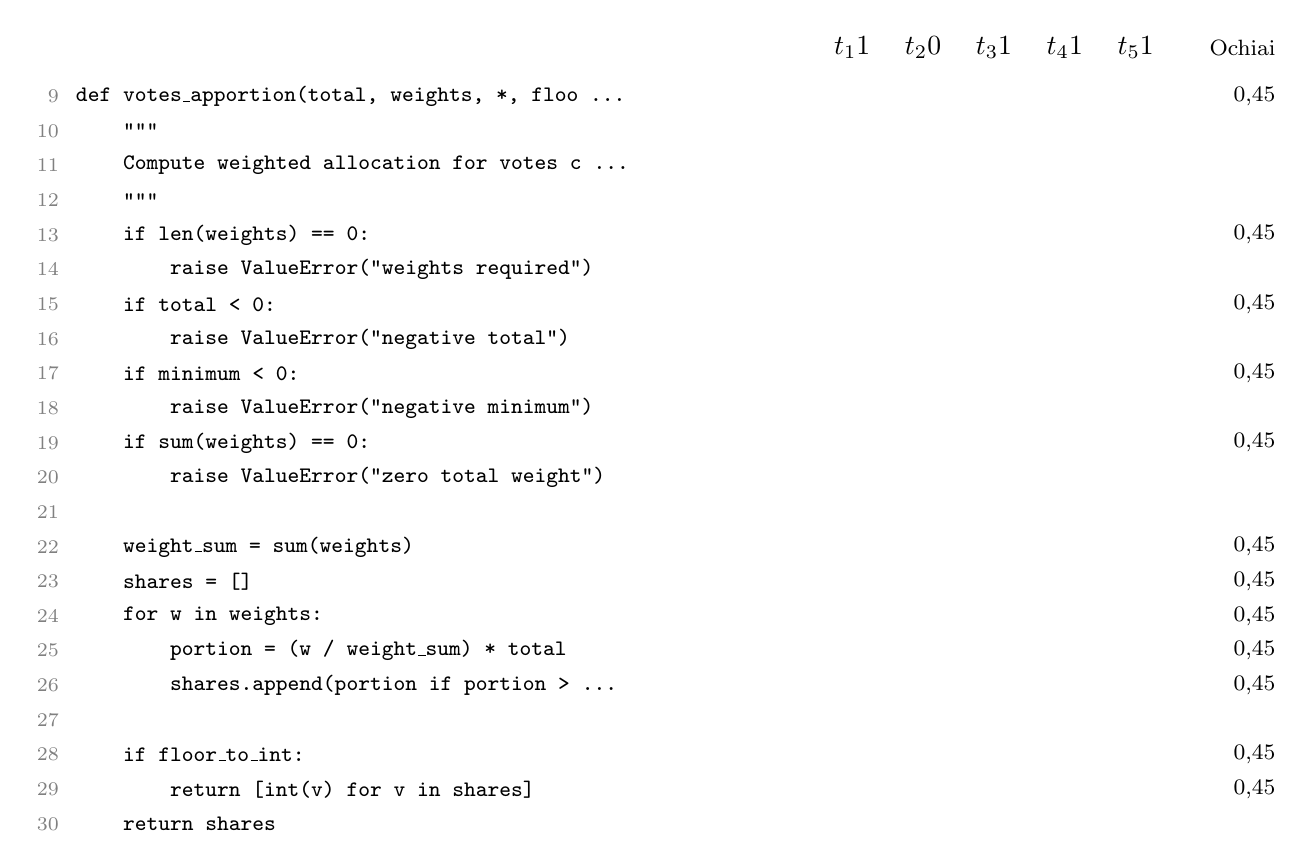
\begin{tikzpicture}[x=1cm, y=-1mm]
\node at (10.40, 0) {\testhead{$t_{1}$}{1}};
\node at (11.30, 0) {\testhead{$t_{2}$}{0}};
\node at (12.20, 0) {\testhead{$t_{3}$}{1}};
\node at (13.10, 0) {\testhead{$t_{4}$}{1}};
\node at (14.00, 0) {\testhead{$t_{5}$}{1}};
\node[anchor=east] at (15.90, 0) {\footnotesize Ochiai};
\node[anchor=east, font=\scriptsize\color{gray}] at (0.45, 6.16) {9};
\node[anchor=west, font=\ttfamily\footnotesize, inner sep=1pt] at (0.5, 6.16) {def votes\_apportion(total, weights, *, floo …};
\node at (10.40, 6.16) {\covdot};
\node at (11.30, 6.16) {\covdot};
\node at (12.20, 6.16) {\covdot};
\node at (13.10, 6.16) {\covdot};
\node at (14.00, 6.16) {\covdot};
\node[anchor=east, font=\footnotesize] at (15.90, 6.16) {0,45};
\node[anchor=east, font=\scriptsize\color{gray}] at (0.45, 10.56) {10};
\node[anchor=west, font=\ttfamily\footnotesize, inner sep=1pt] at (0.5, 10.56) {\hspace*{2.0em}"""};
\node[anchor=east, font=\scriptsize\color{gray}] at (0.45, 14.96) {11};
\node[anchor=west, font=\ttfamily\footnotesize, inner sep=1pt] at (0.5, 14.96) {\hspace*{2.0em}Compute weighted allocation for votes c …};
\node[anchor=east, font=\scriptsize\color{gray}] at (0.45, 19.36) {12};
\node[anchor=west, font=\ttfamily\footnotesize, inner sep=1pt] at (0.5, 19.36) {\hspace*{2.0em}"""};
\node[anchor=east, font=\scriptsize\color{gray}] at (0.45, 23.76) {13};
\node[anchor=west, font=\ttfamily\footnotesize, inner sep=1pt] at (0.5, 23.76) {\hspace*{2.0em}if len(weights) == 0:};
\node at (10.40, 23.76) {\covdot};
\node at (11.30, 23.76) {\covdot};
\node at (12.20, 23.76) {\covdot};
\node at (13.10, 23.76) {\covdot};
\node at (14.00, 23.76) {\covdot};
\node[anchor=east, font=\footnotesize] at (15.90, 23.76) {0,45};
\node[anchor=east, font=\scriptsize\color{gray}] at (0.45, 28.16) {14};
\node[anchor=west, font=\ttfamily\footnotesize, inner sep=1pt] at (0.5, 28.16) {\hspace*{4.0em}raise ValueError("weights required")};
\node[anchor=east, font=\scriptsize\color{gray}] at (0.45, 32.56) {15};
\node[anchor=west, font=\ttfamily\footnotesize, inner sep=1pt] at (0.5, 32.56) {\hspace*{2.0em}if total < 0:};
\node at (10.40, 32.56) {\covdot};
\node at (11.30, 32.56) {\covdot};
\node at (12.20, 32.56) {\covdot};
\node at (13.10, 32.56) {\covdot};
\node at (14.00, 32.56) {\covdot};
\node[anchor=east, font=\footnotesize] at (15.90, 32.56) {0,45};
\node[anchor=east, font=\scriptsize\color{gray}] at (0.45, 36.96) {16};
\node[anchor=west, font=\ttfamily\footnotesize, inner sep=1pt] at (0.5, 36.96) {\hspace*{4.0em}raise ValueError("negative total")};
\node[anchor=east, font=\scriptsize\color{gray}] at (0.45, 41.36) {17};
\node[anchor=west, font=\ttfamily\footnotesize, inner sep=1pt] at (0.5, 41.36) {\hspace*{2.0em}if minimum < 0:};
\node at (10.40, 41.36) {\covdot};
\node at (11.30, 41.36) {\covdot};
\node at (12.20, 41.36) {\covdot};
\node at (13.10, 41.36) {\covdot};
\node at (14.00, 41.36) {\covdot};
\node[anchor=east, font=\footnotesize] at (15.90, 41.36) {0,45};
\node[anchor=east, font=\scriptsize\color{gray}] at (0.45, 45.76) {18};
\node[anchor=west, font=\ttfamily\footnotesize, inner sep=1pt] at (0.5, 45.76) {\hspace*{4.0em}raise ValueError("negative minimum")};
\node[anchor=east, font=\scriptsize\color{gray}] at (0.45, 50.16) {19};
\node[anchor=west, font=\ttfamily\footnotesize, inner sep=1pt] at (0.5, 50.16) {\hspace*{2.0em}if sum(weights) == 0:};
\node at (10.40, 50.16) {\covdot};
\node at (11.30, 50.16) {\covdot};
\node at (12.20, 50.16) {\covdot};
\node at (13.10, 50.16) {\covdot};
\node at (14.00, 50.16) {\covdot};
\node[anchor=east, font=\footnotesize] at (15.90, 50.16) {0,45};
\node[anchor=east, font=\scriptsize\color{gray}] at (0.45, 54.56) {20};
\node[anchor=west, font=\ttfamily\footnotesize, inner sep=1pt] at (0.5, 54.56) {\hspace*{4.0em}raise ValueError("zero total weight")};
\node[anchor=east, font=\scriptsize\color{gray}] at (0.45, 58.96) {21};
\node[anchor=west, font=\ttfamily\footnotesize, inner sep=1pt] at (0.5, 58.96) {};
\node[anchor=east, font=\scriptsize\color{gray}] at (0.45, 63.36) {22};
\node[anchor=west, font=\ttfamily\footnotesize, inner sep=1pt] at (0.5, 63.36) {\hspace*{2.0em}weight\_sum = sum(weights)};
\node at (10.40, 63.36) {\covdot};
\node at (11.30, 63.36) {\covdot};
\node at (12.20, 63.36) {\covdot};
\node at (13.10, 63.36) {\covdot};
\node at (14.00, 63.36) {\covdot};
\node[anchor=east, font=\footnotesize] at (15.90, 63.36) {0,45};
\node[anchor=east, font=\scriptsize\color{gray}] at (0.45, 67.76) {23};
\node[anchor=west, font=\ttfamily\footnotesize, inner sep=1pt] at (0.5, 67.76) {\hspace*{2.0em}shares = []};
\node at (10.40, 67.76) {\covdot};
\node at (11.30, 67.76) {\covdot};
\node at (12.20, 67.76) {\covdot};
\node at (13.10, 67.76) {\covdot};
\node at (14.00, 67.76) {\covdot};
\node[anchor=east, font=\footnotesize] at (15.90, 67.76) {0,45};
\node[anchor=east, font=\scriptsize\color{gray}] at (0.45, 72.16) {24};
\node[anchor=west, font=\ttfamily\footnotesize, inner sep=1pt] at (0.5, 72.16) {\hspace*{2.0em}for w in weights:};
\node at (10.40, 72.16) {\covdot};
\node at (11.30, 72.16) {\covdot};
\node at (12.20, 72.16) {\covdot};
\node at (13.10, 72.16) {\covdot};
\node at (14.00, 72.16) {\covdot};
\node[anchor=east, font=\footnotesize] at (15.90, 72.16) {0,45};
\node[anchor=east, font=\scriptsize\color{gray}] at (0.45, 76.56) {25};
\node[anchor=west, font=\ttfamily\footnotesize, inner sep=1pt] at (0.5, 76.56) {\hspace*{4.0em}portion = (w / weight\_sum) * total};
\node at (10.40, 76.56) {\covdot};
\node at (11.30, 76.56) {\covdot};
\node at (12.20, 76.56) {\covdot};
\node at (13.10, 76.56) {\covdot};
\node at (14.00, 76.56) {\covdot};
\node[anchor=east, font=\footnotesize] at (15.90, 76.56) {0,45};
\node[anchor=east, font=\scriptsize\color{gray}] at (0.45, 80.96) {26};
\node[anchor=west, font=\ttfamily\footnotesize, inner sep=1pt] at (0.5, 80.96) {\hspace*{4.0em}shares.append(portion if portion > …};
\node at (10.40, 80.96) {\covdot};
\node at (11.30, 80.96) {\covdot};
\node at (12.20, 80.96) {\covdot};
\node at (13.10, 80.96) {\covdot};
\node at (14.00, 80.96) {\covdot};
\node[anchor=east, font=\footnotesize] at (15.90, 80.96) {0,45};
\node[anchor=east, font=\scriptsize\color{gray}] at (0.45, 85.36) {27};
\node[anchor=west, font=\ttfamily\footnotesize, inner sep=1pt] at (0.5, 85.36) {};
\node[anchor=east, font=\scriptsize\color{gray}] at (0.45, 89.76) {28};
\node[anchor=west, font=\ttfamily\footnotesize, inner sep=1pt] at (0.5, 89.76) {\hspace*{2.0em}if floor\_to\_int:};
\node at (10.40, 89.76) {\covdot};
\node at (11.30, 89.76) {\covdot};
\node at (12.20, 89.76) {\covdot};
\node at (13.10, 89.76) {\covdot};
\node at (14.00, 89.76) {\covdot};
\node[anchor=east, font=\footnotesize] at (15.90, 89.76) {0,45};
\gtrow{94.16}{16.00}
\node[anchor=east, font=\scriptsize\color{gray}] at (0.45, 94.16) {29};
\node[anchor=west, font=\ttfamily\footnotesize, inner sep=1pt] at (0.5, 94.16) {\hspace*{4.0em}return [int(v) for v in shares]};
\node at (10.40, 94.16) {\covdot};
\node at (11.30, 94.16) {\covdot};
\node at (12.20, 94.16) {\covdot};
\node at (13.10, 94.16) {\covdot};
\node at (14.00, 94.16) {\covdot};
\node[anchor=east, font=\footnotesize] at (15.90, 94.16) {0,45};
\node[anchor=east, font=\scriptsize\color{gray}] at (0.45, 98.56) {30};
\node[anchor=west, font=\ttfamily\footnotesize, inner sep=1pt] at (0.5, 98.56) {\hspace*{2.0em}return shares};
\end{tikzpicture}
}

\caption{SBFL không phân biệt được dòng lỗi của một lỗi ngữ nghĩa. Chương trình \texttt{votes\_apportion} (SemFault-250, tập test): mỗi cột là một kiểm thử, chấm là kiểm thử đó chạy qua dòng. Kiểm thử thất bại và kiểm thử thành công chạy qua đúng cùng các dòng, nên mọi dòng có cùng điểm Ochiai; dòng tô màu là dòng lỗi (nhãn đã chuẩn hóa)}
\label{fig:sbfl-mu}
\end{figure}

\label{sec:tinh-dong}%
Phân tích tĩnh (ruff, pyrefly) chỉ biết mã \emph{được viết} thế nào, không biết mã \emph{được mong đợi} làm gì: viết
\texttt{>} thay cho \texttt{>=} vẫn hợp lệ về cú pháp và kiểu. Với lỗi ngữ nghĩa, chỉ kiểm thử chứa ý định của lập
trình viên, nên định vị lỗi thuộc về phân tích động; phân tích tĩnh chỉ là mốc so sánh.

\section{SemLoc: phổ vi phạm ràng buộc ngữ nghĩa}
\label{sec:semloc}

SemLoc~\cite{yang2026semloc} (Hình~\ref{fig:semloc}) cho LLM viết các ràng buộc ngữ nghĩa, chèn mỗi ràng buộc vào
chương trình thành một lệnh kiểm tra và chạy bộ kiểm thử để có ma trận ``ràng buộc $\times$ kiểm thử''; áp
công thức~\eqref{eq:ochiai} lên ma trận này cho điểm của từng ràng buộc. Điểm này được nhân với hệ số theo loại vị trí (gắn vào đúng một dòng: \ConstRegionWeightLine; cuối nhánh
\texttt{if}: \ConstRegionWeightAfterBranch; cuối vòng lặp: \ConstRegionWeightLoopTail; mọi lệnh \texttt{return}:
\ConstRegionWeightAnyReturn), và điểm của một dòng là giá trị lớn nhất trong các ràng buộc gắn với nó. Bước kiểm chứng
phản thực tế loại ràng buộc bị vi phạm cả trong kiểm thử thành công, rồi cho LLM vá thử tại dòng của từng ràng buộc còn
lại và chạy lại kiểm thử.

\begin{figure}[H]
\centering
{\setstretch{1}%
\begin{tikzpicture}[node distance=4mm and 6mm, font=\small, arr/.style={-{Stealth[length=2mm]}},
  box/.style={draw, rounded corners, align=center, minimum height=11mm, text width=24mm, fill=blue!4},
  ours/.style={draw=orange!80!black, dashed, rounded corners, align=center, minimum height=11mm, text width=30mm, font=\footnotesize, fill=orange!6}]
\node[box] (a) {Chương trình\\+ kiểm thử}; \node[box, right=of a] (b) {LLM sinh\\ràng buộc};
\node[box, right=of b] (c) {Chèn mã,\\chạy kiểm thử}; \node[box, right=of c] (d) {Phổ vi phạm\\(Ochiai)};
\node[box, below=10mm of d] (e) {Kiểm chứng\\phản thực tế}; \node[box, left=of e] (f) {Xếp hạng\\dòng};
\node[ours, left=of f] (g) {+\ConstPriorWeight{} điểm cho dòng LLM\\tự đoán (không có\\trong bài báo)};
\draw[arr] (a) -- (b); \draw[arr] (b) -- (c); \draw[arr] (c) -- (d); \draw[arr] (d) -- (e); \draw[arr] (e) -- (f);
\draw[arr, dashed, orange!80!black] (b) -- (b |- g.north); \draw[arr, dashed, orange!80!black] (g) -- (f);
\end{tikzpicture}}
\caption{Quy trình của SemLoc (theo~\cite{yang2026semloc}); khung nét đứt là thành phần nhóm phát hiện trong mã nguồn}
\label{fig:semloc}
\end{figure}

\textbf{Điểm thưởng cho dòng LLM tự đoán.} Mã nguồn công khai có một thành phần không được mô tả trong bài báo: ngoài
các ràng buộc, LLM còn trả về một dòng lỗi nó tự đoán (trường \texttt{fault\_line}), và dòng này được cộng thêm
\ConstPriorWeight{} điểm, lớn hơn điểm tối đa 1 của một ràng buộc. Vì vậy dòng LLM tự đoán \emph{luôn} đứng hạng 1, bất
kể phổ vi phạm ra sao (Hình~\ref{fig:diem-thuong}); đây là trọng tâm của câu hỏi ``grounded hay guessed''.
Hình~\ref{fig:semloc-blend} đi qua từng bước trên \texttt{blend\_orders}. Ở
\texttt{votes\_apportion} (Hình~\ref{fig:sbfl-mu}), không ràng buộc nào LLM viết bị vi phạm, nên mọi điểm phổ bằng 0 và
hạng 1 của SemLoc (dòng 26, không phải dòng lỗi) hoàn toàn do điểm thưởng.

\begin{figure}[H]
\centering
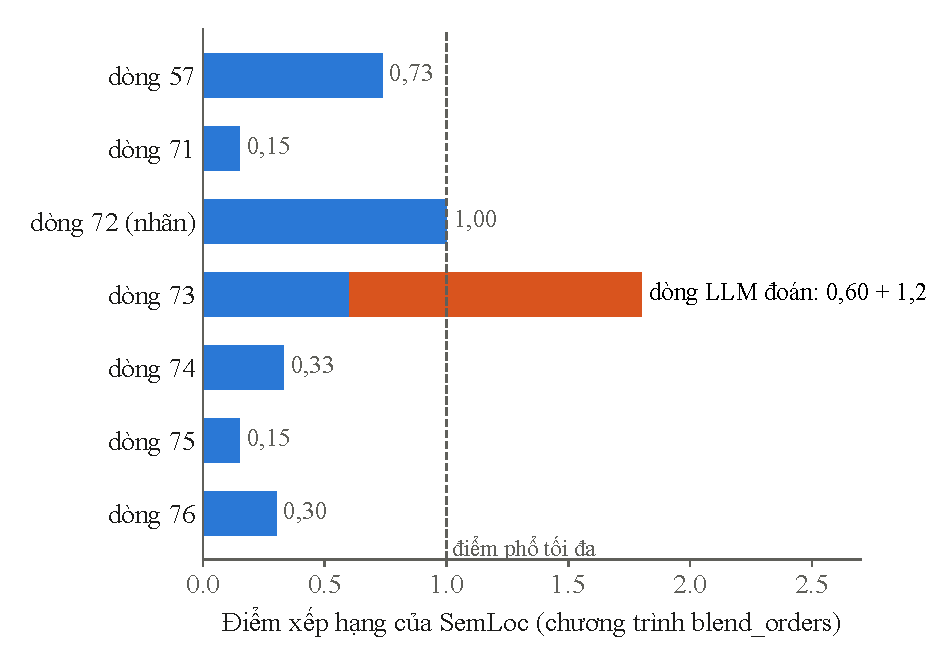
\includegraphics{../generated/vi/fig_semloc_bonus.pdf}
\caption{Điểm xếp hạng của SemLoc trên từng dòng của một chương trình (lượt chạy 1, Gemini 3.8 Flash). Phần xanh là điểm phổ vi phạm, tối đa là 1; phần cam là điểm thưởng \ConstPriorWeight{} mà mã nguồn công bố cộng cho dòng LLM tự đoán. Dòng nhãn có điểm phổ cao nhất nhưng dòng đoán vẫn vượt lên hạng 1}
\label{fig:diem-thuong}
\end{figure}
\begin{figure}[H]
\centering
{\small\setstretch{1.05}
\begin{tabular}{@{}r>{\raggedright\arraybackslash}p{0.86\linewidth}@{}}
\toprule
Dòng & Mã nguồn (dòng nghiêng: kiểm tra được SemLoc chèn vào) \\
\midrule
70 & \texttt{\hspace*{2.0em}merged.extend(\_clamp\_value(v) for v in right[j:])} \\
71 & \texttt{} \\
\rowcolor{failloc!12}72 & \texttt{\hspace*{2.0em}if merged and left and right and merged[-1] == left[-1] == right[-1]:} \\
 & \textit{\color{semloc}kiểm tra C2: \texttt{len(merged\_\_1) == len(left) + len(right)}} \\
73 & \texttt{\hspace*{4.0em}merged.pop()} \\
 & \textit{\color{semloc}kiểm tra C1: \texttt{len(merged\_\_1) == len(left) + len(right)}} \\
74 & \texttt{} \\
75 & \texttt{\hspace*{2.0em}\_log.debug("Blended \%d + \%d orders into \%d total", len(left), len(right), …} \\
\bottomrule
\end{tabular}

\medskip
\begin{tabularx}{\linewidth}{@{}lp{1.5cm}>{\raggedright\arraybackslash}X>{\centering\arraybackslash}p{1.2cm}>{\centering\arraybackslash}p{1.2cm}>{\centering\arraybackslash}p{1.2cm}>{\centering\arraybackslash}p{1.2cm}>{\centering\arraybackslash}p{1.2cm}@{}}
\toprule
Ràng buộc & Gắn ở & Biểu thức & Kiểm thử thất bại vi phạm & Kiểm thử thành công vi phạm & Ochiai & Hệ số vùng & Điểm cho dòng \\
\midrule
C1 & 73 & \texttt{len(merged\_\_1) == len(left) + len(right)} & 4 & 0 & 1,00 & 0,6 & 0,60 \\
C2 & 72 & \texttt{len(merged\_\_1) == len(left) + len(right)} & 4 & 0 & 1,00 & 1,0 & 1,00 \\
C3 & loop tail & \texttt{len(merged\_\_1) == i + j} & 4 & 2 & 0,82 & 0,9 & 0,73 \\
C4 & any return & \texttt{len(\_\_cbfl\_result) == len(left) + len(right)} & 4 & 0 & 1,00 & 0,3 & 0,30 \\
\bottomrule
\end{tabularx}

\medskip
Điểm xếp hạng: dòng 73: 0,60 + 1,2 (hạng 1); dòng 72: 1,00 (hạng 2); dòng 57: 0,73 (hạng 3).}

\caption{SemLoc trên chương trình \texttt{blend\_orders} (lượt chạy 1, Gemini 3.8 Flash; dòng tô màu là dòng lỗi theo nhãn đã chuẩn hóa). Trên: mã nguồn với các lệnh kiểm tra được chèn. Giữa: số kiểm thử thất bại và kiểm thử thành công vi phạm từng ràng buộc và điểm Ochiai. Dưới: điểm xếp hạng của ba dòng đầu}
\label{fig:semloc-blend}
\end{figure}

% nội dung 1 của thầy: tài liệu, từ khóa, nghiên cứu liên quan
\section{Tổng quan tài liệu và khoảng trống nghiên cứu}
\label{sec:tim-tai-lieu}\label{chap:tong-quan}

Điểm xuất phát là ba bài giảng viên giao cho chương~10 ``Phát hiện lỗi và định vị lỗi''.
Nhóm lần ngược tài liệu được trích dẫn và tìm xuôi nghiên cứu mới trên arXiv, ACM DL, IEEE Xplore và Google Scholar,
chọn các phương pháp SemLoc so sánh hay kế thừa, bộ dữ liệu lỗi Python, và các bài về cách đánh giá, rủi ro khi dùng LLM,
nhãn sai và bản sửa ``lách'' kiểm thử. Bảng~\ref{tab:tu-khoa} là bộ từ khóa song ngữ dùng để tìm và thống nhất thuật ngữ.

\begin{table}[H]
\centering
\caption{Bộ từ khóa của đề tài}
\label{tab:tu-khoa}
\small
\begin{tabular}{@{}ll@{}}
\toprule
Tiếng Anh & Tiếng Việt \\
\midrule
fault localization & định vị lỗi \\
spectrum-based fault localization (SBFL) & định vị lỗi dựa trên phổ độ phủ \\
semantic fault & lỗi ngữ nghĩa \\
semantic constraint / invariant & ràng buộc ngữ nghĩa / bất biến \\
semantic violation spectrum & phổ vi phạm ràng buộc ngữ nghĩa \\
counterfactual verification & kiểm chứng phản thực tế \\
large language model (LLM) & mô hình ngôn ngữ lớn \\
structured grounding & neo lập luận vào biểu diễn có cấu trúc \\
program instrumentation & chèn mã kiểm tra vào chương trình \\
reproducibility & tính tái hiện được \\
data contamination / memorization & nhiễm dữ liệu huấn luyện / ghi nhớ \\
omission fault & lỗi thiếu mã \\
test-driven development (TDD) & phát triển hướng kiểm thử \\
plausible patch / test overfitting & bản sửa hợp lệ bề ngoài / quá khớp kiểm thử \\
label error (benchmark) & nhãn sai trong bộ dữ liệu \\
static / dynamic analysis & phân tích tĩnh / phân tích động \\
\bottomrule
\end{tabular}
\end{table}

\label{sec:ba-bai-bao}%
\textbf{SemLoc}~\cite{yang2026semloc} nhắm vào lỗi ngữ nghĩa, nơi phổ độ phủ ``sụp''. Phương pháp (Mục~\ref{sec:semloc}) gồm bốn bước: tìm điểm
neo (đầu hàm, định nghĩa -- sử dụng, biên vòng lặp, lệnh trả về); một lượt gọi LLM sinh ràng buộc gắn với điểm neo; chèn
ràng buộc, chạy kiểm thử, chấm ma trận ``ràng buộc $\times$ kiểm thử'' bằng Ochiai; vá thử một dòng để kiểm chứng phản
thực tế. Trên SemFault-250 (250 chương trình Python một hàm, một lỗi) bài báo báo cáo Acc@1
\RqOneSemlocClaudeTZeroEightAuthorAllAccOne\%, nhưng chỉ có kết quả cấp dòng cho bảy lỗi thật. Mã chấm điểm phá hòa theo
thứ tự dòng, loại chương trình chạy lỗi khỏi mẫu số, mỗi cấu hình chạy một lần; đây là đầu vào của RQ1.

\textbf{EffiHolmes}~\cite{yang2026effiholmes} định vị lỗi hiệu năng, loại lỗi không làm kiểm thử thất bại: chạy chương
trình ở hai mức tải, coi hàm có chi phí tăng theo tải là điểm nóng và cho LLM lập luận trên đường gọi tới đó (140 vấn
đề thật). Nhóm học ý tưởng \emph{đối chiếu hai lần thực thi để lọc nhiễu} (nền của CovGate) và khuôn câu hỏi nghiên cứu.

\textbf{Báo cáo sự cố kết hợp LLM}~\cite{medeiros2026crash} gom cụm vết ngăn xếp của hai hệ thống Java công nghiệp, xếp
hạng phương thức đáng nghi rồi đưa vào prompt; trên 38 lỗi thật, cấu hình tốt nhất định vị được 71/100. Bài học: đưa
bằng chứng đã khai thác vào prompt giúp LLM (ý tưởng của biến thể có độ phủ từng dòng), và đầu ra LLM cần được kiểm tra.

\label{sec:khoang-trong}%
Về định vị lỗi, Ochiai~\cite{abreu2009} là mốc SBFL chuẩn, với hai điểm yếu đánh giá đã biết là hòa điểm và lỗi thiếu
mã~\cite{wong2016survey}; gỡ lỗi chia đôi~\cite{zeller2002tse} là nền cho bước kiểm chứng của SemLoc. Trong định vị lỗi
bằng LLM, AutoFL~\cite{kang2024autofl} và FlexFL~\cite{xu2025flexfl} đưa bằng chứng thực thi vào prompt, Wu và cộng
sự~\cite{wu2023llmfl} thấy nhật ký lỗi giúp LLM rõ rệt, còn Agentless~\cite{xia2024agentless} cho thấy quy trình đơn
giản có thể thắng tác tử phức tạp. Về tính hợp lệ, cách chấm~\cite{pearson2017} và nhãn sai~\cite{northcutt2021labels}
đều có thể đảo thứ hạng, bản sửa vượt kiểm thử thường không đúng~\cite{qi2015kali}, và LLM có thể đã ghi nhớ bộ dữ
liệu~\cite{ramos2024memorize}. Bảng~\ref{tab:so-sanh-tai-lieu} đặt ba bài cạnh hướng của nhóm. Khoảng trống còn lại: chưa ai đo phần độ chính xác thật
sự đến từ bằng chứng thực thi; kết quả SemLoc đến từ một lần chạy với cách chấm lạc quan trên nhãn chưa kiểm tra; và
chưa có so sánh với cách làm đơn giản mà lập trình viên vẫn dùng, tức một prompt có kiểm thử thất bại. Bốn câu hỏi nghiên
cứu ở Chương~\ref{chap:mo-dau} lấp ba khoảng trống này.

\begin{table}[H]
\centering
\caption{So sánh ba bài báo được giao với hướng của nhóm}
\label{tab:so-sanh-tai-lieu}
\small
\begin{tabularx}{\linewidth}{@{}>{\raggedright\arraybackslash}p{0.17\linewidth}*{4}{>{\raggedright\arraybackslash}X}@{}}
\toprule
Tiêu chí & SemLoc~\cite{yang2026semloc} & EffiHolmes~\cite{yang2026effiholmes} & Báo cáo sự cố + LLM~\cite{medeiros2026crash} & Nhóm M9 \\
\midrule
Loại lỗi & ngữ nghĩa & hiệu năng & sự cố (Java) & ngữ nghĩa \\
Tín hiệu & ràng buộc do LLM sinh + chạy kiểm thử & phân tích hiệu năng ở hai mức tải & vết ngăn xếp + xếp hạng & kiểm thử thất bại đưa thẳng cho LLM; tách đóng góp của từng tín hiệu \\
Lỗi thật & 7 lỗi có kết quả cấp dòng & 140 vấn đề & 38 lỗi công nghiệp & 31 lỗi BugsInPy, 3 lần chạy \\
Kiểm tra bộ dữ liệu & không & --- & --- & kiểm chứng bằng thực thi và rà soát toàn bộ nhãn \\
Lặp và kiểm định & 1 lần, không kiểm định & --- & --- & 3 lần, McNemar, bootstrap theo cụm \\
\bottomrule
\end{tabularx}
\end{table}
